\documentclass[manuscript,review]{acmart}

\setcopyright{none}
\acmConference{}
\acmYear{2026}
\acmDOI{}
\acmISBN{}
\settopmatter{printacmref=false}
\renewcommand\footnotetextcopyrightpermission[1]{}
 \usepackage{placeins}
 
\title{LLMs Get Lost In Multi-Turn Conversation}
 
\author{Philippe Laban}
\affiliation{
    \institution{Microsoft Research}
    \country{USA}
}
\email{plaban@microsoft.com}

\author{Hiroaki Hayashi}
\affiliation{
    \institution{Salesforce Research}
    \country{USA}
}
\email{hiroakihayashi@salesforce.com}

\author{Yingbo Zhou}
\affiliation{
    \institution{Salesforce Research}
    \country{USA}
}
\email{yingbo.zhou@salesforce.com}

\author{Jennifer Neville}
\affiliation{
    \institution{Microsoft Research}
    \country{USA}
}
\email{jenneville@microsoft.com}

\begin{document}


\begin{abstract}
Large Language Models (LLMs) are conversational interfaces. As such, LLMs
have the potential to assist their users not only when they can fully specify the task
at hand, but also to help them define, explore, and refine what they need through
multi-turn conversational exchange. Although analysis of LLM conversation logs
has confirmed that underspecification occurs frequently in user instructions, LLM
evaluation has predominantly focused on the single-turn, fully-specified instruction
setting. In this work, we perform large-scale simulation experiments to compare
LLM performance in single- and multi-turn settings. Our experiments confirm
that all the top open- and closed-weight LLMs we test exhibit significantly lower
performance in multi-turn conversations than single-turn, with an average drop of
39\% across six generation tasks. Analysis of 200,000+ simulated conversations
decomposes the performance degradation into two components: a minor loss in
aptitude and a significant increase in unreliability. We find that LLMs often make
assumptions in early turns and prematurely attempt to generate final solutions, on
which they overly rely. In simpler terms, we discover that when LLMs take a
wrong turn in a conversation, they get lost and do not recover.

\begin{figure}[htbp]
    \centering
    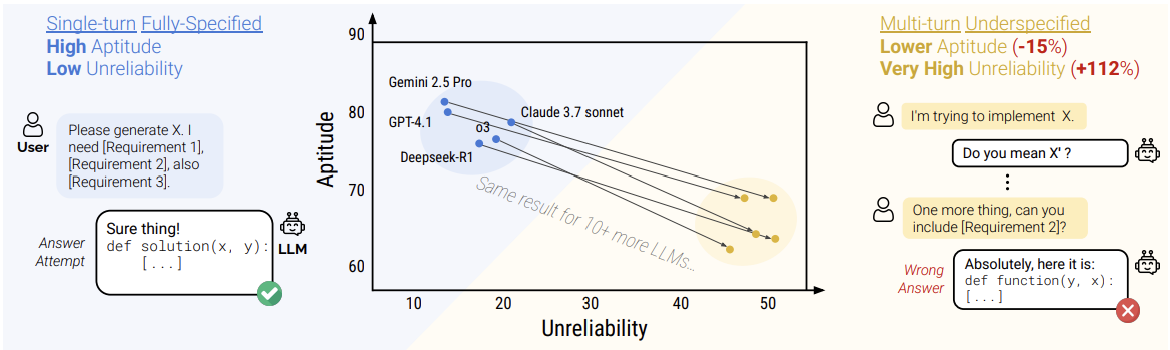
\includegraphics[width=0.85\textwidth]{Figure_1.png}
    \caption{Simulated conversations for 6 generation tasks on the 15 LLMs that observe a major
performance drop in multi-turn settings (-39\%), explained by some loss in Aptitude, and large loss in
Reliability}
    \label{fig:figure_1_abstract}
\end{figure}

\end{abstract}

\maketitle

\section{Introduction}

Modern Large Language Model (LLM) architectures, including commercial platforms such as ChatGPT, Gemini, and Claude, are inherently engineered to function as conversational agents across extended, multi-turn dialogues rather than static, one-shot question-answering engines. This architectural paradigm is critical because real-world users rarely formulate fully-specified requirements in their initial query. Instead, human-AI interactions typically commence with incomplete, underspecified instructions, with users progressively introducing parameters, constraints, and operational details as the conversation unfolds. Empirical analyses of production dialogue logs confirm that this form of task \emph{underspecification} represents the operational norm \cite{herlihy2024overcoming}. Despite this reality, the standard benchmarking ecosystem remains overwhelmingly preoccupied with single-turn evaluations, wherein a model is evaluated based on its response to a singular, comprehensively detailed prompt. This methodological discrepancy introduces a severe disconnect between laboratory evaluation metrics and practical deployment performance.

Furthermore, existing multi-turn evaluation frameworks frequently adopt an flawed conceptual premise: they treat ongoing dialogue as an \emph{episodic} sequence of independent, self-contained sub-tasks. Under this episodic framework, individual conversational turns are graded in isolation, operating under the assumption that a model's capacity to resolve consecutive sub-tasks implies overarching multi-turn competence. This paper demonstrates that such a framing fails to capture the defining challenge of multi-turn interaction—specifically, the cognitive demand to accumulate, track, and reconcile disparate informational constraints distributed across an entire conversational trajectory. This non-episodic, incremental delivery of information is deeply rooted in human communication patterns, historically formalized in linguistics as the ``principle of least effort'' \cite{zipf1949human}, which notes that speakers naturally minimize initial informational output.

To systematically analyze this evaluation gap, the authors implement an algorithmic simulation pipeline designated as \textbf{sharded simulation}. The core mechanism of this framework involves taking high-quality, fully-specified evaluation instances from verified single-turn benchmarks and mechanically partitioning them into distinct informational units, or \emph{shards}. Each shard represents an isolated instruction component that a user might realistically provide in a single conversational turn. A simulated user agent then systematically introduces these shards to the target LLM one turn at a time, adhering to natural dialogue flow. Consequently, the model only obtains the complete problem specification upon the arrival of the final shard. This methodology uniquely allows the researchers to leverage established, reliable evaluation metrics while isolating and comparing single-turn versus multi-turn performance on identical underlying tasks.

Executing this simulation pipeline at scale—encompassing over 200,000 simulated dialogues across 15 prominent open- and closed-weight LLMs across six distinct generation domains—reveals a striking, systemic vulnerability. Every evaluated model exhibits severe performance degradation when instruction parameters are distributed across multiple turns compared to when they are presented monolithically, demonstrating an average performance drop of approximately 39\%. Crucially, analytical breakdowns indicate that this decline is not primarily caused by a deficiency in the models' underlying \emph{aptitude} when executing fragmented tasks. Instead, the degradation is driven by a massive escalation in model \emph{unreliability}: the identical model, evaluated on the identical task split across turns, can yield completely correct outputs on one run and entirely erroneous results on another. The authors formalize this as a failure mode where the model gets ``lost'' after adopting an incorrect assumption in early turns, rendering it incapable of recovery even when subsequent turns explicitly provide the required corrective data.

The paper systematically investigates the behavioral root causes driving this multi-turn failure, identifying several recurring pathology patterns. First, models demonstrate a strong bias toward excessive verbosity, producing long responses that clutter the context window. Second, models consistently display an over-eager tendency to generate full, definitive solutions prematurely before receiving sufficient task specifications, thereby embedding unverified assumptions into the dialogue history. Third, once an incorrect assumption is written into the context, the model exhibits an architectural over-reliance on its own past generations, failing to discard invalid context when newer, conflicting constraints arrive. Given that this failure mode spans both compact open-weight models and frontier-scale systems, the authors frame this as a critical, unaddressed reliability bottleneck in current AI alignment. The study concludes with practical, actionable mitigation strategies tailored for LLM providers, application developers, and end-users.


\section{Background and Related Work}

The authors situate their work relative to two generations of conversational NLP research. Older
generation models such as BART, GPT-2, and T5 were originally designed and evaluated for single-turn
tasks; when developers wanted an actual dialogue agent, they typically built one as a modular pipeline
that used a language model as just one component, and evaluated the resulting system through human
studies rather than automatic multi-turn benchmarks.
 
Since the rise of ChatGPT, a newer line of work has proposed evaluating LLMs directly in multi-turn
settings. The authors' central critique of this line of work is that it largely still frames a
conversation as \emph{episodic}: each turn is treated as an independent sub-task that can be scored on its
own, without requiring the model to combine information spread across multiple turns. The paper argues
that this framing significantly overstates how well models actually handle multi-turn interaction, because
in practice users routinely under-specify their requests both when talking to AI systems
\cite{herlihy2024overcoming} and in everyday human conversation \cite{zipf1949human}. The authors place
this kind of underspecification -- rather than merely ``multiple turns'' -- at the center of their study.
 
A second issue the authors raise with prior multi-turn benchmarks is a mismatch in task granularity: the
sub-tasks used to test multi-turn ability are often different in nature from the single-turn tasks used
elsewhere, which makes it hard to directly compare single- and multi-turn performance on equal footing.
The sharded-simulation approach in this paper is explicitly designed to close that gap by deriving both
the single-turn and multi-turn versions of a task from the very same original instruction. The paper also
narrows its scope to open-ended generation tasks (e.g., writing code, generating SQL, producing a
summary) rather than short-form classification or extraction tasks, arguing that generation is both the
predominant real-world usage pattern for LLMs and the setting in which underspecification is most
consequential, since a partially-specified generation task can be quietly ``completed'' with an incorrect
assumption in a way that a classification task usually cannot.

\begin{figure}[htbp]
    \centering
    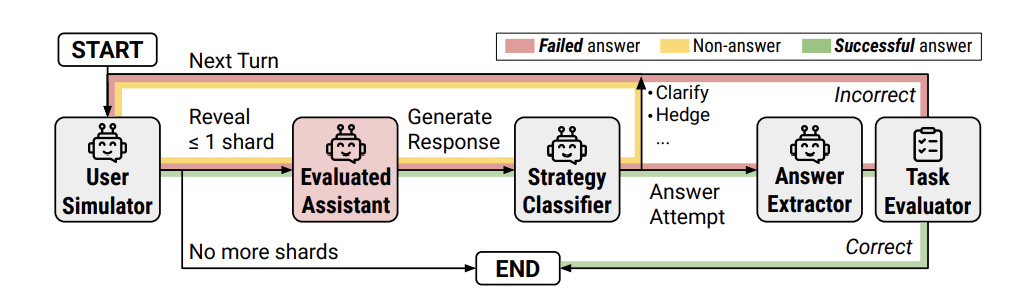
\includegraphics[width=0.85\textwidth]{Figure_2.png}
    \caption{Sharded Conversation Simulation Diagram. The simulation subject is highlighted in red.}
    \label{fig:figure_2_background}
\end{figure}
 
Simulating a user is itself a design decision with trade-offs. The paper notes that prior work has explored
a spectrum of options, from rule-based templates, to LLM-driven simulated users, to fixed human annotations,
to studies with real human participants -- each trading off cost and scalability against realism. The
authors adopt an LLM-based simulated user (a smaller model, GPT-4o-mini) because it is inexpensive enough
to run at the scale of hundreds of thousands of conversations while still being able to select and phrase
shards contextually, e.g., answering a clarification question with the relevant piece of information rather
than revealing shards in a rigid, pre-determined order. The authors are explicit that this simulated user
is a simplification and should be read as a controlled probe of \emph{assistant} behavior, not as a
faithful model of how real people write; they argue in their limitations discussion that this choice, if
anything, likely makes their reported degradation numbers an \emph{underestimate} of what would occur with
real, less predictable human users.


 
\section{Method}
 
\subsection{Turning single-turn instructions into shards}
The paper's central methodological contribution is a process for converting an existing, fully-specified instruction $q$ (with a known correct answer) into a \emph{sharded instruction}: an ordered set of short, conversational shards $[s_1, \ldots, s_k]$ that, taken together, convey the same information as the original instruction. For a sharded instruction $q'$ to be considered valid for an original query $q$, the authors require it to satisfy several properties defined in Appendix B:
\begin{itemize}
    \item \textbf{P1: Information Preservation ($I(q) = I(q')$):} No information from the original instruction necessary for the completion of the instruction should be lost during the sharding process.
    \item \textbf{P2: Clear Initial Intent ($I_q = I_{q'}$ and $s_1 = I_q$):} The first shard must clearly establish the high-level goal of the task (e.g., ``write a Python function''), so that the conversation has a coherent starting point.
    \item \textbf{P3: Order Insensitive:} Shards other than the first should not depend on one another for their meaning, so that revealing them in a different order still conveys the same overall information. Let $\rho(s_{2..k})$ refer to a permutation of the shard ordering, then $I(q) = I(\tilde{q}) \quad \forall \tilde{q} = [s_1, \rho(s_{2..k})]$.
    \item \textbf{P4: Maximal Sharding:} The shards should be split as finely as reasonably possible, each introducing a single new piece of information (maximizing $k$).
    \item \textbf{P5: Minimal Transformation:} The sharded instruction should maintain the instruction language and avoid simplifying, altering, or interpreting elements of the original instruction as much as possible.
\end{itemize}
 
To produce shards that satisfy these properties at scale, the authors use a four-step, semi-automatic pipeline: (1) \textbf{Segmentation}, where an LLM is prompted to break the original instruction into non-overlapping segments, each intended to correspond to one atomic piece of information; instructions that yield fewer than three segments are discarded as too simple to usefully shard; (2) \textbf{Rephrasing}, where each segment is rewritten into a short, self-contained, conversational shard, and one segment is chosen and rephrased to serve as the natural opening message of the conversation; (3) \textbf{Verification}, where the authors run preliminary simulations comparing the original instruction against a single-turn reconstruction built by concatenating all shards together, and discard any sharded instruction whose reconstructed performance falls too far below the original (a check meant to catch cases where information was accidentally lost or the shards secretly depend on being read in a fixed order); and (4) \textbf{manual inspection}, where the authors personally review, edit, merge, or reject every candidate sharded instruction to guarantee a consistently high level of quality across the final dataset.
 


\subsection{Simulating a Conversation}
 
Once a sharded instruction exists, the authors simulate a conversation between the model under test (the \emph{assistant}) and an LLM-driven \emph{user simulator} (instantiated via GPT-4o-mini) that owns the full shard set and decides, turn by turn, which shard to reveal next. Rather than disclosing shards in a rigid or random sequence, the user simulator dynamically selects and lightly rephrases the shard that best fits the immediate exchange, such as responding directly to an assistant's clarification request with the relevant parameter constraint. A separate LLM-based \emph{strategy classifier} labels every assistant turn into one of seven categories adapted from prior work \cite{herlihy2024overcoming} -- for example, asking a clarifying question, hedging with multiple hypothetical answers, refusing to answer, or making a full \emph{answer attempt}. 

Whenever a turn is classified as an answer attempt, an \emph{answer extractor} pulls out just the answer portion of the response (e.g., a code block or a number) and passes it to a task-specific evaluator reused from the original benchmark the instruction was drawn from. Because the assistant may attempt an answer more than once over the course of a conversation, its final score for a sharded conversation is simply the best score obtained across all of its attempts -- a design choice that, if anything, gives the assistant a slight structural advantage compared to the strictly single-shot single-turn setting. Before the first turn, the assistant is given only minimal, task-appropriate context (such as a list of available tools) and is never told that the conversation will be underspecified or span multiple turns, so that the experiment measures the model's default, unprompted behavior.
 
The same underlying shards can be recombined into several different conversation formats, which the paper uses to isolate different possible causes of performance degradation:
\textsc{Full} presents the original, fully-specified instruction in a single turn and serves as the upper-bound baseline; \textsc{Concat} presents all shards concatenated into one bulleted message in a single turn, which controls for whether the act of \emph{rephrasing} content into shard form (rather than multi-turn delivery itself) explains any performance loss; \textsc{Sharded} is the core underspecified multi-turn condition described above; \textsc{Recap} runs a full \textsc{Sharded} conversation and then adds one final turn that restates every shard at once, testing whether a simple, agent-style reminder at the end can undo the damage; and \textsc{Snowball} instead re-states all previously revealed shards at \emph{every} turn as the conversation progresses, testing whether continual repetition throughout the conversation (rather than only at the end) reduces the burden on the model's memory.


\subsection{Tasks, models, and metrics}
 
The authors build sharded instructions for six generation tasks, each derived from an established,
high-quality single-turn benchmark, spanning both programming and natural-language use cases: writing a
Python function (from HumanEval \cite{chen2021evaluating} and LiveCodeBench), writing a SQL query given a
database schema (from Spider \cite{yu2018spider}), generating API calls that satisfy a request (from the
Berkeley Function Calling Leaderboard \cite{yan2024bfcl}), solving an elementary math word problem (from
GSM8K \cite{cobbe2021training}), captioning a table (from ToTTo \cite{parikh2020totto}), and writing a
cited multi-document summary (from Summary of a Haystack \cite{laban2024summary}). Figure~\ref{fig:tasks}
shows an example fully-specified instruction and its sharded counterpart for each of the six tasks. Between
90 and 120 valid sharded instructions were produced per task after the four-step pipeline and manual
review described above. Each task reuses the exact-match, functional-accuracy, or BLEU-style metric from
its original benchmark, mapped onto a common 0--100 scale so that results can be aggregated and compared
across tasks.

\begin{figure*}[t]
  \centering
  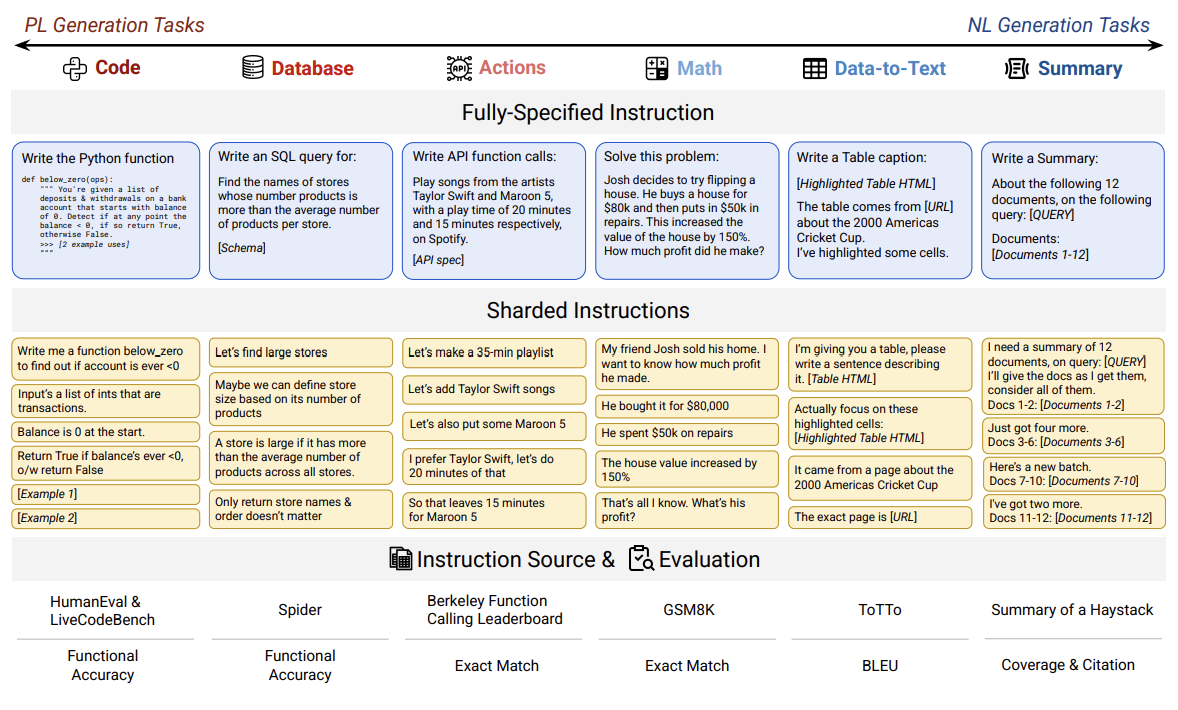
\includegraphics[width=0.92\linewidth]{Figure_4.png}
  \caption{Six sharded tasks included in the experiments. The tasks cover both programming and natural language generation paradigms. For each task, an illustrative fully-specified instruction and its sharded counterpart are provided, drawn from an initial pool of 90 to 120 instructions per benchmark domain. Reproduced from the original paper (Figure 4) \cite{laban2025llmslost}.}
  \label{fig:tasks}
\end{figure*}
 
Fifteen LLMs spanning eight model families were evaluated, deliberately chosen to cover a wide capability
and scale range: small open-weight models (e.g., Llama-3.1-8B-Instruct), mid-sized and large open-weight
models (e.g., Llama-3.3-70B, Command-A), and frontier closed-weight models (e.g., GPT-4.1, Claude 3.7
Sonnet, Gemini 2.5 Pro), plus two reasoning-oriented models (OpenAI's o3 and DeepSeek-R1) included
specifically to test whether extra test-time compute helps a model avoid getting lost in conversation. For
the main experiment, each (model, task, simulation-type) combination was run ten times at the default
sampling temperature, since LLM generation is stochastic and repeated sampling is required to measure how
much a model's output quality varies from run to run for the same underlying instruction. From these
repeated runs the authors define three per-instruction metrics: \textbf{averaged performance}
, the mean score across the ten runs; \textbf{aptitude}, the 90th-percentile
score, intended as a best-case estimate of what the model is capable of; and \textbf{unreliability}
, the gap between the 90th- and 10th-percentile scores, intended to capture how much quality
swings from run to run purely due to randomness. Framed this way, a large drop in average performance
between the \textsc{Full} and \textsc{Sharded} settings can in principle be explained by a genuine loss in
capability (lower aptitude), by increased run-to-run inconsistency (higher unreliability), or by some
combination of the two -- and separating these two explanations is the main goal of the paper's analysis in Section~\ref{sec:results}.


 
\section{Findings and Results}
\label{sec:results}

\subsection{Average Performance Degrades Sharply and Consistently}
 
Across all fifteen models and all six tasks, every single model performs significantly worse in the \textsc{Sharded} setting than in the \textsc{Full} setting, with an average performance drop of roughly 39\%. The authors call this the \emph{Lost in Conversation} effect: models that comfortably score above 90\% when handed a complete instruction up front struggle heavily on the exact same underlying problems once that information is spread across a short, natural back-and-forth dialogue. 

Crucially, performance in the \textsc{Concat} condition—where all the rephrased shards are given together at once—remains highly stable, retaining about 95\% of the baseline \textsc{Full} performance. Because \textsc{Concat} isolates the structural impact of rephrasing without spreading it over time, this stability proves that the sharp drop in the \textsc{Sharded} setting is not a side effect of how the shards were worded. Instead, it is caused specifically by delivering the specifications incrementally across multiple turns. As illustrated by the trends in Figure~\ref{fig:figure_1_abstract} back in the abstract, this conversational breakdown splits into two distinct behavioral flaws: while the models experience a noticeable 15\% drop in baseline aptitude, the true driver of failure is a massive 112\% surge in unreliability.
 
Somewhat counter-intuitively, this performance collapse is not confined to smaller or weaker open-weight models. High-capacity, frontier-scale systems like Claude 3.7 Sonnet, GPT-4.1, and the Gemini 2.5 family lose roughly the same 30--40\% of their performance as considerably smaller models like Llama-3.1-8B-Instruct. While some of this uniform percentage drop is linked to baseline ceiling effects—weaker models simply have less room to fall since they start with a lower initial score—the core takeaway holds steady: single-turn proficiency offers no real guarantee of multi-turn conversational robustness. 

The severity of the drop does, however, vary by task and model domain. Command-A handles the multi-turn API-calling task relatively well, whereas Claude 3.7 Sonnet and GPT-4.1 hold onto their performance best on programming tasks. This highlights that multi-turn resilience is not a single, uniform property of a model but relies heavily on the type of task being performed. Interestingly, adding test-time compute through reasoning models like o3 or DeepSeek-R1 does not fix this underlying vulnerability either; both reasoners degrade in a pattern remarkably similar to standard models of comparable strength. The authors attribute this to the fact that reasoning models generate longer responses on average, which clutters the history and increases the risk of getting lost in long context windows.
 
Table~\ref{tab:overall} details these patterns by showing each model's average performance in the \textsc{Concat} and \textsc{Sharded} settings, normalized as a percentage of its original \textsc{Full}-turn baseline score across all six tasks.
 
\begin{table}[t]
  \centering
  \caption{Average performance in the \textsc{Concat} and \textsc{Sharded} settings, expressed as a percentage of each model's own \textsc{Full}-setting baseline performance, averaged across the six tasks. Models are listed in ascending order of their baseline single-turn performance.}
  \label{tab:overall}
  \begin{tabular}{lrr}
    \toprule
    \textbf{Model} & \textbf{Concat / Full (\%)} & \textbf{Sharded / Full (\%)} \\
    \midrule
    Llama-3.1-8B-Instruct & 91.6 & 62.5 \\
    OLMo2-13B             & 86.5 & 50.5 \\
    Claude 3 Haiku         & 91.6 & 52.4 \\
    GPT-4o-mini             & 93.0 & 56.2 \\
    Llama-3.3-70B-Instruct  & 93.2 & 64.2 \\
    Phi-4                   & 99.0 & 61.7 \\
    Command-A               & 97.3 & 60.4 \\
    Llama-4-Scout            & 91.0 & 66.1 \\
    o3                       & 98.1 & 64.1 \\
    Claude 3.7 Sonnet         & 100.4 & 65.9 \\
    DeepSeek-R1               & 103.6 & 60.8 \\
    GPT-4o                     & 94.5 & 57.9 \\
    Gemini 2.5 Flash            & 99.3 & 65.8 \\
    GPT-4.1                     & 97.9 & 61.8 \\
    Gemini 2.5 Pro                & 100.1 & 64.5 \\
    \bottomrule
  \end{tabular}
\end{table}
 
Two primary insights stand out from the data in Table~\ref{tab:overall}. First, every evaluated model retains nearly all of its baseline capability when processing the shards all at once in the \textsc{Concat} setting (with minor variations slightly above 100\% due to baseline stochastic sampling noise), reinforcing that rephrasing alone does not disrupt model understanding. Second, when the same information is introduced sequentially via the \textsc{Sharded} framework, every single model's performance plunges into a tight window between roughly 50\% and 66\% of its baseline score. This uniform drop highlights a complete lack of correlation between foundational single-turn strength and conversational endurance: compact open-weight configurations and massive frontier systems ultimately scale down to the exact same vulnerable performance envelope when forced to navigate multi-turn context updates.

Ultimately, these findings show that the true bottleneck in multi-turn interactions isn't a lack of raw capability. Instead, the process of handling information bit by bit forces even the most advanced models into a state of high unpredictability. Once a model is forced to adapt to shifting constraints over time, its single-turn reliability completely fractures, leaving it highly vulnerable to getting permanently derailed as the conversation moves forward.



\subsection{Why Models Fail: Consistent Ability vs. Unpredictable Performance}
 
The paper's most important analytical contribution is decomposing this performance drop into two distinct components: aptitude ($A^{90}$) and unreliability ($U_{10}^{90}$). In a single-turn setting, these two metrics behave exactly how you would expect. High-performing models like GPT-4.1 and Gemini 2.5 Pro deliver the best of both worlds—they achieve high best-case scores alongside very low run-to-run variance. Conversely, weaker models are both less capable overall and far less consistent.

\begin{figure}[htbp]
    \centering
    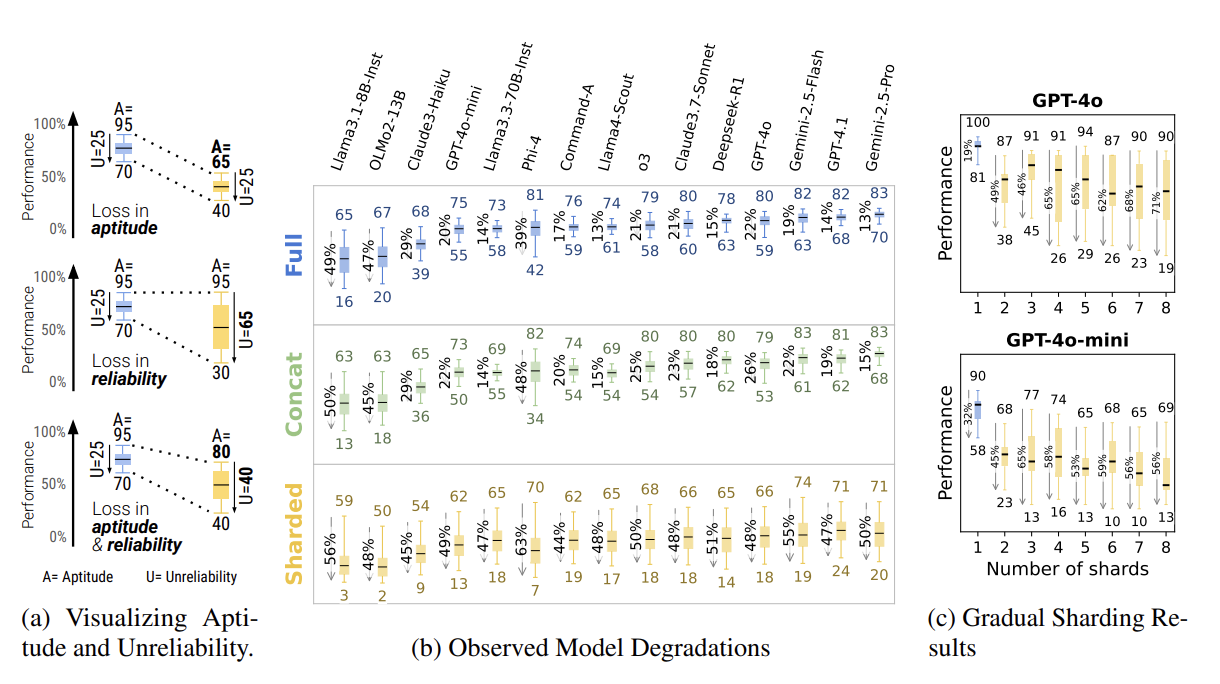
\includegraphics[width=0.85\textwidth]{Figure_5.png}
    \caption{Visualizing Aptitude and Unreliability as box-plot statistics: the top of the upper whisker marks aptitude, while the gap between the upper and lower whiskers marks unreliability. Reproduced from the original paper (Figure 5a) \cite{laban2025llmslost}.}
    \label{fig:figure_5_aptitude}
\end{figure}

 
However, that intuitive relationship completely breaks down in the \textsc{Sharded} setting. Interestingly, a model's foundational aptitude only dips modestly between the \textsc{Full} and \textsc{Sharded} conditions—dropping by about 16\% on average. This means that in their best simulated runs, the models are still nearly as capable as they are in a single-turn setup. 

Instead, the real culprit is a massive spike in unreliability, which more than doubles with an average increase of roughly 112\%. This volatility impacts every single model across the board; on the exact same instruction, the gap between a model's best-case and worst-case runs widens by about 50 percentage points. Ultimately, this reveals that the \emph{Lost in Conversation} effect is overwhelmingly a reliability problem rather than a lack of raw capability. When information is delivered across several turns instead of one, the exact same model becomes highly unpredictable—solving a task perfectly on one attempt, only to fail it entirely on the next.


\subsection{Why Models Get Lost and How the Number of Turns Affects Them}
\label{sec:causes}
 
By looking closely at the conversation transcripts, the authors found four common habits that explain why these models suddenly become so unreliable:

First, models are often way too eager. They try to give a final, complete answer right at the beginning of the chat before they even have enough information to go on. This premature guessing forces the model to make assumptions. Unfortunately, once it locks into a wrong guess early on, it rarely corrects itself later. In fact, chats where the model waits a bit longer before making its first real answer attempt score much higher on average than chats where it jumps the gun, as shown in Table~\ref{tab:timing}.

\begin{table}[t]
  \centering
  \caption{Averaged performance based on how early in the conversation the model makes its first answer attempt, measured on the Code and Math tasks. Scores climb steadily the longer a model waits before committing to an answer.}
  \label{tab:timing}
  \begin{tabular}{lrrrrr}
    \toprule
    \textbf{Model} & \textbf{0--20\%} & \textbf{20--40\%} & \textbf{40--60\%} & \textbf{60--80\%} & \textbf{80--100\%} \\
    \midrule
    Llama-3.1-8B  & 16.1 & 24.0 & 35.3 & 39.6 & 39.7 \\
    Claude 3 Haiku & 27.1 & 35.6 & 47.4 & 58.9 & 70.3 \\
    GPT-4o-mini    & 30.2 & 39.2 & 48.4 & 58.2 & 59.9 \\
    Command-A      & 38.0 & 42.9 & 56.5 & 65.5 & 73.5 \\
    Claude 3.7 Sonnet & 29.2 & 35.6 & 55.3 & 68.0 & 71.6 \\
    GPT-4.1        & 33.9 & 52.7 & 60.6 & 69.0 & 78.6 \\
    Gemini 2.5 Pro & 41.1 & 45.7 & 53.5 & 64.6 & 63.8 \\
    \midrule
    \textbf{Average (15 models)} & \textbf{30.9} & \textbf{40.5} & \textbf{51.7} & \textbf{60.4} & \textbf{64.4} \\
    \bottomrule
  \end{tabular}
\end{table}

The pattern holds for every model tested: an answer attempted in the first 20\% of the conversation averages only 30.9\% correctness, compared to 64.4\% when the model holds off until the final 20\%---roughly double the score, simply by waiting.

Second, when the model makes later attempts to fix its answer, those responses get noticeably longer than its usual single-turn answers. The authors call this ``answer bloat.'' Instead of wiping the slate clean and starting fresh, the model tends to stack new fixes right on top of its old, incorrect assumptions, cluttering its own memory.

Third, in tasks that require summarizing documents with citations, the models show a strong bias. They mostly pay attention to documents brought up in the very first turn or the absolute most recent turn, almost entirely ignoring what happened in the middle of the chat. This is a conversational version of the well-known ``lost-in-the-middle'' problem \cite{liu2024lost} often seen in long single-turn prompts.

Fourth, simply writing a longer response makes things worse. Across almost all tasks, longer answers are tied to lower scores. The more the model talks, the more likely it is to accidentally introduce unstated assumptions that clash with what the user actually asked for later.

A separate experiment looked at whether the size of the informational chunks mattered. The authors took the instructions and split them into different versions, ranging from just two turns up to eight turns, using GPT-4o and GPT-4o-mini. Interestingly, both models showed the exact same drop in reliability the moment an instruction was split into just two turns. Breaking the task down into even more turns did not make the performance drop noticeably worse. This proves that the core issue isn't how finely you chop up the information; simply moving from a single prompt to a conversation with more than one turn is enough to cause the model to lose its footing.

Finally, the authors tried two simple fixes that don't require rewriting or retraining the models. In the \textsc{Recap} setup, they added a final turn where the user reminds the model of every requirement mentioned so far. In the more realistic \textsc{Snowball} setup, every single user turn automatically repeats all previous requirements alongside the new one. While both ideas helped recover some lost ground—with \textsc{Snowball} closing about 15--20\% of the performance gap—neither came close to matching the high scores of the original single-turn baseline. Lowering the model's creativity settings (sampling temperature) to zero or adding a warning in the system prompt did not help much either. Ultimately, this shows that multi-turn unreliability is a deep, structural problem within the models themselves, and it cannot be easily fixed with clever prompting tricks.

\FloatBarrier

\subsection{Lowering Temperature Does Not Fix Multi-Turn Unreliability}

A natural question is whether simply making the model's output more deterministic---by
lowering the sampling temperature---would resolve the reliability problem outright. The
authors tested this directly on GPT-4o and GPT-4o-mini, varying both the assistant's
temperature and, since the user is itself simulated by an LLM, the user simulator's
temperature as well, across three settings each: 1.0, 0.5, and 0.0.

\begin{table}[htbp]
  \centering
  \caption{Unreliability ($U_{10}^{90}$) of GPT-4o under different assistant (AT) and user (UT) sampling temperatures. Lower values indicate more reliable behavior. In single-turn settings (Full, Concat), reliability improves sharply as temperature drops; in the Sharded setting, it barely moves.}
  \label{tab:temperature}
  \begin{tabular}{lrrr}
    \toprule
    \textbf{Setting} & \textbf{AT=1.0} & \textbf{AT=0.5} & \textbf{AT=0.0} \\
    \midrule
    Full           & 17.8 & 8.0  & 2.8 \\
    Concat         & 20.2 & 17.8 & 5.8 \\
    \midrule
    Sharded (UT=1.0) & 41.0 & 43.8 & 31.8 \\
    Sharded (UT=0.5) & 39.5 & 40.8 & 31.8 \\
    Sharded (UT=0.0) & 35.8 & 38.0 & 29.7 \\
    \bottomrule
  \end{tabular}
\end{table}

Table~\ref{tab:temperature} shows the result. In the single-turn settings, dropping the
temperature to zero collapses unreliability almost entirely, exactly as one would expect
from more deterministic decoding. In the \textsc{Sharded} setting, however, unreliability
barely improves, and stays stubbornly high at around 30\% even when both the assistant
and the simulated user are set to temperature zero. The authors attribute this to the fact
that modern LLMs are not perfectly deterministic even at $T=0$, due to floating-point
non-determinism in the underlying hardware; a single early token flip can cascade into a
completely different conversational trajectory several turns later, an effect that simply
does not have time to compound within a single-turn response. In short, unreliability in
multi-turn conversation is not just sampling noise that a lower temperature can dial away---it
is a structural consequence of errors compounding over turns.

\section{Discussion}
 
Taken together, these results show that we need a major shift in how we measure the quality of Large Language Models. A model's single-turn benchmark score, no matter how impressive, simply cannot predict how reliably that same model will perform in the real world, where instructions usually arrive gradually and with key details missing. Breaking the performance drop down into aptitude and unreliability is perhaps the most useful contribution of this study. It gives researchers a clear, actionable target—reducing run-to-run inconsistency when details are missing—instead of just pointing out that multi-turn chats are difficult.

The paper outlines important lessons for a few different audiences:

For \textbf{LLM Builders}, the findings emphasize that multi-turn reliability needs to be prioritized just as much as raw capability. The authors set a concrete goal for future models: they should maintain the same aptitude in both single- and multi-turn settings, keep their unreliability metric ($U_{10}^{90}$) below 15 in multi-turn chats, and achieve this at a standard sampling temperature ($T=1$). Interestingly, the experiments prove that simply dropping the temperature to $T=0.0$ does not fix multi-turn volatility; early random variations create a cascading effect that keeps unreliability high at around 30\%.

For \textbf{System and Agent Builders}, who might assume that framework tools like LangChain or AutoGen \cite{wu2023autogen} can easily manage conversation states externally, the \textsc{Recap} and \textsc{Snowball} tests offer a reality check. While repeating past context helps a little bit—with \textsc{Snowball} closing about 15--20\% of the performance gap—neither comes close to a true fix. Even the \textsc{Recap} method, which uses a final corrective turn to inform the model that its prior solutions were wrong before restating all rules in a clean bulleted list, falls short. Similarly, adding an explicit system prompt hint warning the model about the multi-turn setup only yields a minor $+1\%$ performance bump without keeping the model from getting lost. Ultimately, true multi-turn reliability must be built directly into the underlying model, rather than being bolted onto the application layer.

For \textbf{NLP Practitioners}, the study introduces a helpful framework for identifying which tasks are most vulnerable to getting derailed in conversation. These tasks usually share three specific traits: they are generative rather than extractive, complex enough to split into three or more conversational turns, and non-episodic—meaning each new piece of information forces the model to change its entire solution. While the authors encourage researchers to release sharded variants alongside fully specified datasets, they note that the semi-automated sharding pipeline still requires a significant manual commitment of about 3 hours per 100 samples to ensure quality.

For \textbf{Everyday Users}, the authors offer two practical, though temporary, workarounds. First, ``if time allows, try again.'' If a model has clearly lost its way, it is much better to open a brand-new chat and start fresh rather than trying to correct the model in the current thread, since early mistakes tend to stick around. Second, ``consolidate before retrying.'' Users can ask the LLM to combine all scattered notes from a messy chat into a single, comprehensive prompt, and then feed that unified prompt into a completely new conversation to get a much more reliable result.

Of course, the study has its limitations, and the authors are transparent about them. The automated setup represents an ideal, highly controlled environment rather than a true replication of chaotic human interaction. The user simulator follows a rigid protocol: it introduces exactly one clear piece of information per turn, ensures the main objective is clear from the very first sentence, and promises that every necessary requirement is perfectly laid out by the final turn. 

Real human conversations are rarely this clean. Humans suffer from misunderstandings over terminology, change their minds, or give up due to frustration with system failures \cite{wester2024giving}, often pursuing goals that don't even have a feasible solution. Because the simulation strips away these messy realities, it functions as an incredibly forgiving, benign testing ground. Furthermore, the scoring system itself structurally favors the multi-turn setup; because the model gets to make multiple answer attempts across different turns, it can be credited for a lucky early guess or benefit from lenient evaluation. The fact that multi-turn performance still plummets by an average of 39\% despite these massive structural advantages strongly suggests that this degradation is a severe underestimate of how often LLMs get lost when interacting with real, unpredictable human users.

Additionally, the scope of the evaluation is structurally bounded. The user simulator follows a rigid protocol, though more work is needed to approach fully natural user simulation \cite{naous2025towards, dou2025simulating, mehri2025user, ross2025simulating}. Furthermore, the six tasks tested all feature analytical, right-or-wrong solutions evaluated exclusively in English text. It remains an open question whether the same conversational degradation occurs in more open-ended, subjective domains like creative writing \cite{chakrabarty2024creativity}. This was a conscious choice: though there has been some progress on creative writing evaluation, it is still an active area of research \cite{chakrabarty2025advancements}, and how these dynamics play out across multilingual and multimodal environments remains an open direction for future work.

Finaly, ensuring absolute long-term reproducibility for these kinds of multi-turn benchmarks presents a couple of unique challenges. Because the vast majority of the experiments rely on closed-source, API-based language models, future verification is inherently limited by the fact that API providers routinely deprecate and retire older model versions over time. Furthermore, the probabilistic nature of LLMs introduces statistical variance into the conversation tracks. While the authors mitigated this by running each simulated conversation 10 independent times to smooth out the data, scaling up the experimental budget even further remains an open path for future work. To support this ongoing research, the authors plan to release their entire simulation code, sharded instructions, and conversation histories publicly.

\bibliographystyle{ACM-Reference-Format}
\bibliography{references}

\end{document}